 \begin{block}{Question 4}
We used \textbf{Count-min (CM) sketch} (\cite{cm-sketch}). Illustration of the approximation of the aggregate variance:

\begin{figure}
    \centering
    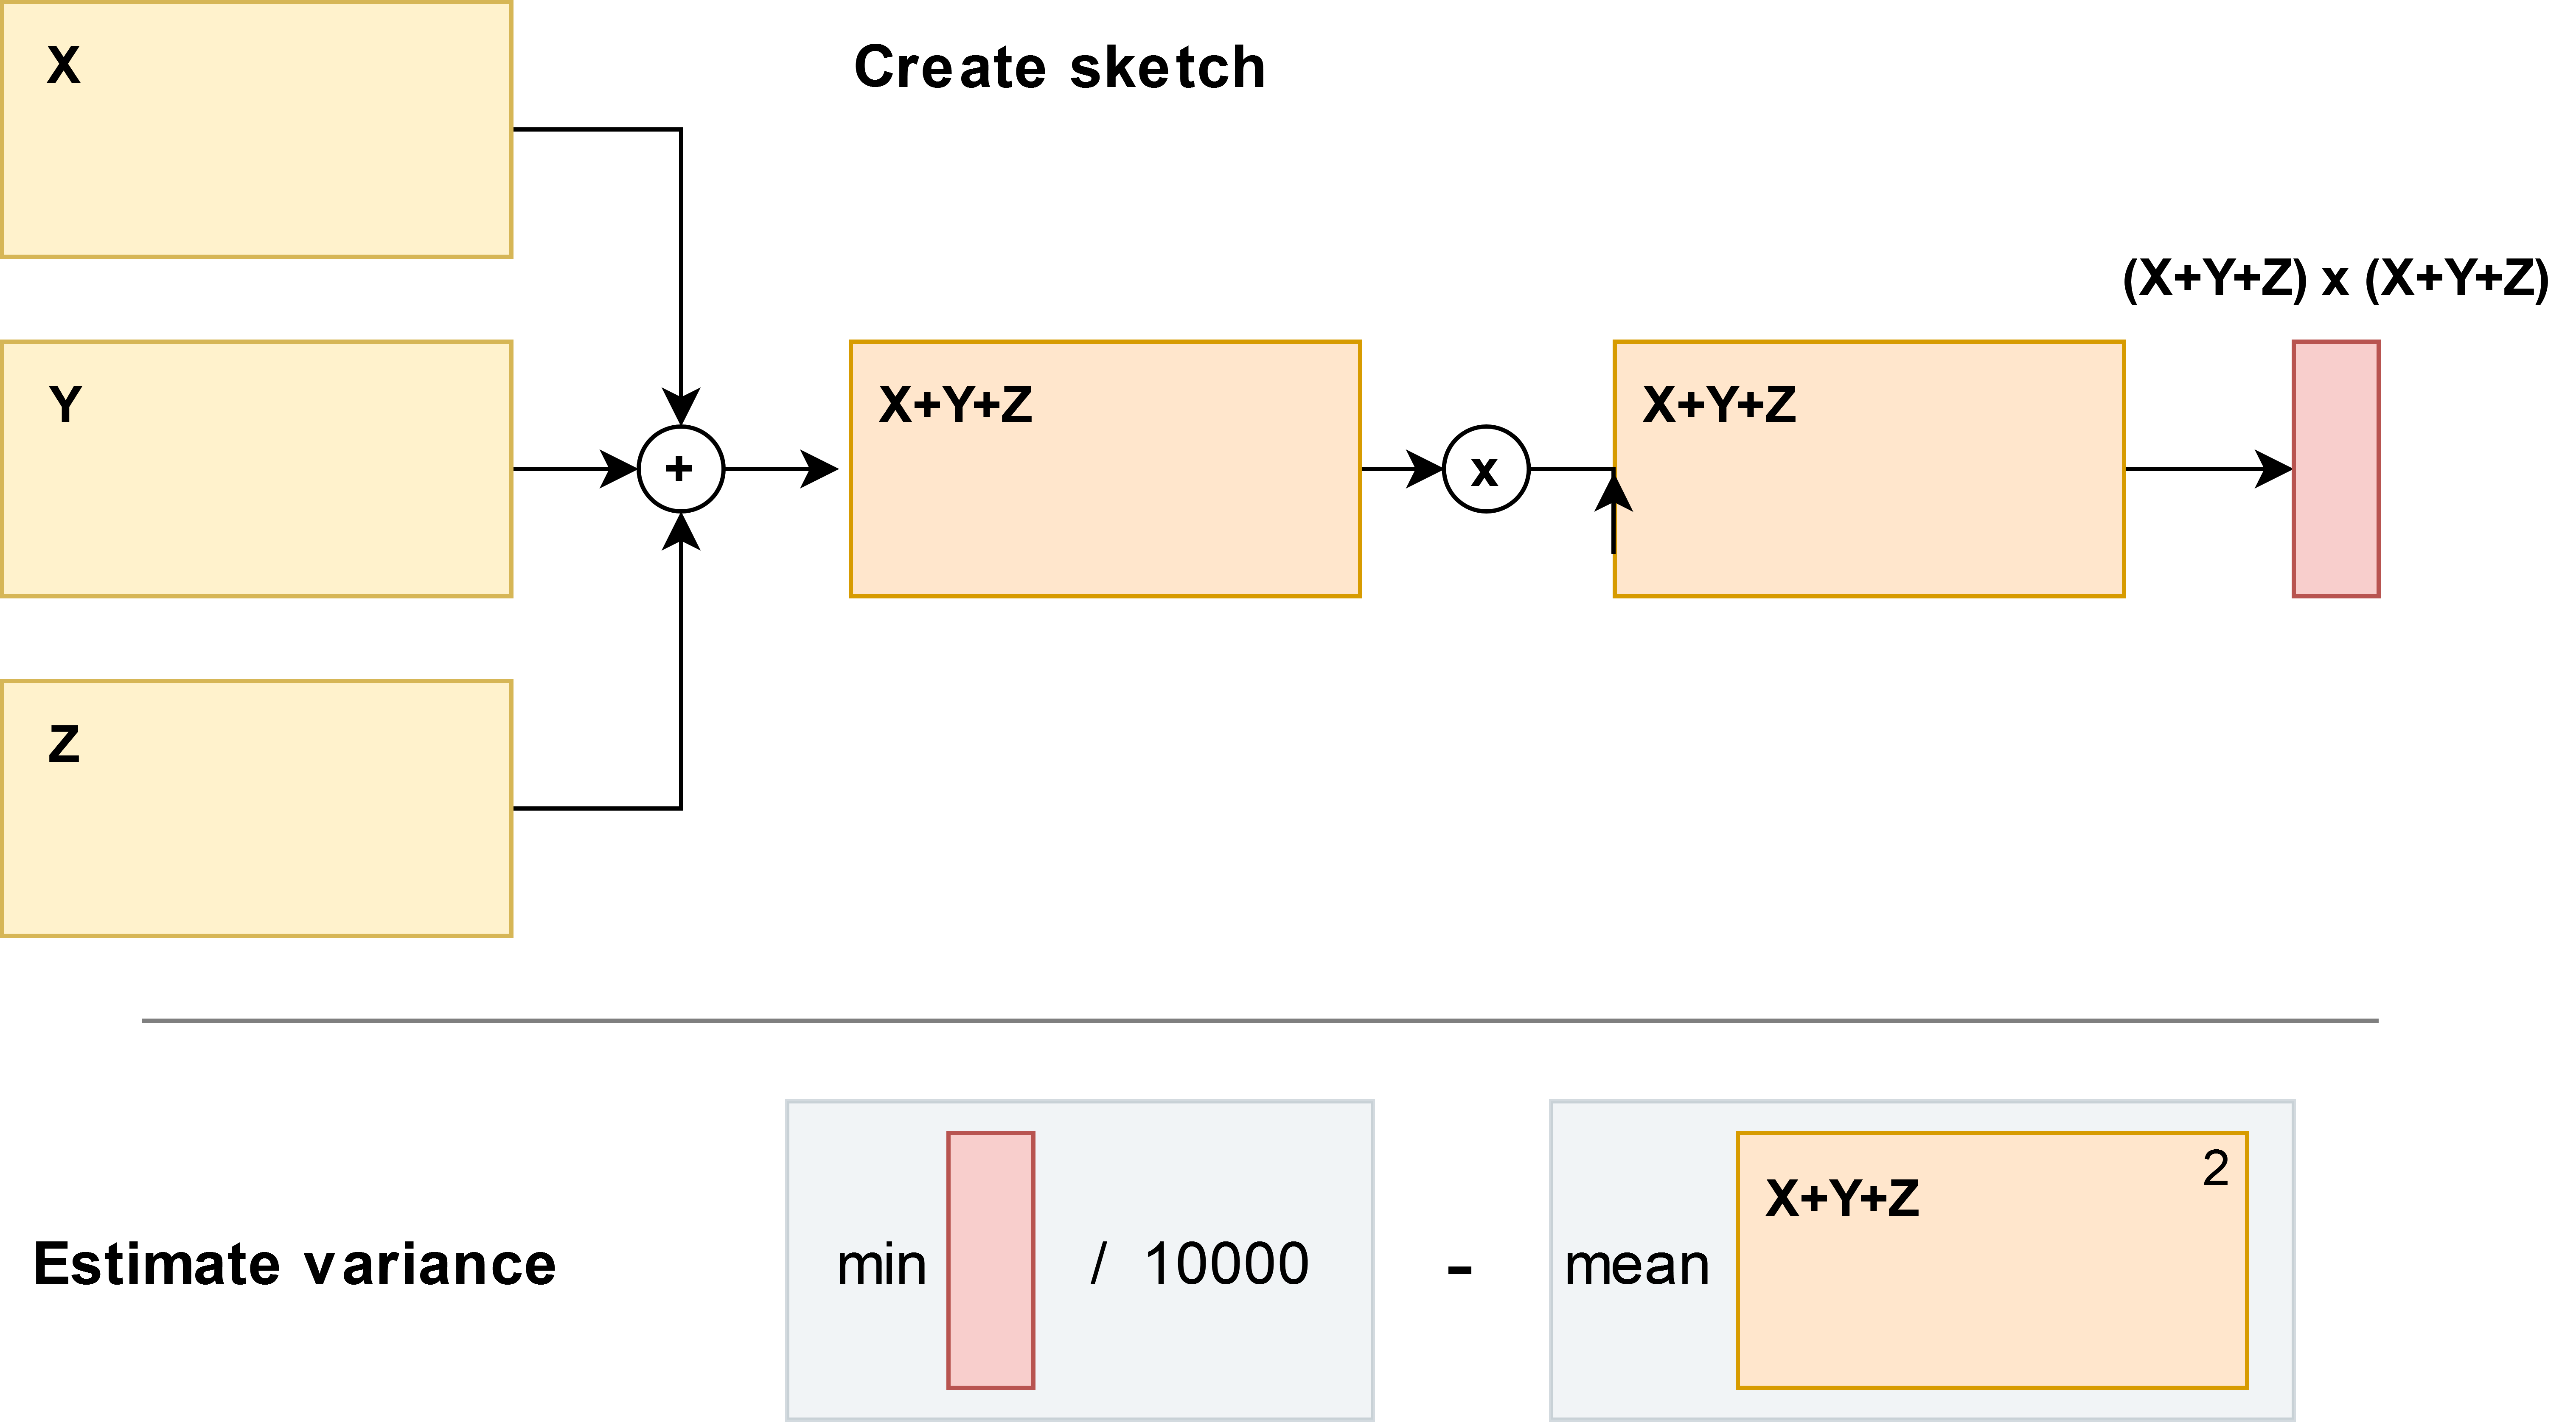
\includegraphics[width=.8\linewidth]{../assets/images/q4_sketch_usage.png}
    \caption{Count-min sketch exploitation for Q4}
    \label{fig:q4_sketch}
\end{figure}

%Formally, the approximated aggregate variance can be expressed as follows,
%\begin{equation}
%    \widehat{\sigma}^2=\left(\frac{1}{10000}\widehat{(\mathbf{a}\odot\mathbf{a})}\right)-\mu_{\mathbf{a}}^2
%\end{equation}

% \begin{columns}[t]
%    \begin{column}{.5\textwidth}
%        \begin{algorithm}[H]
    \label{alg:create_sketch}    
    \caption{Creates CM sketch from vector.}
    \DontPrintSemicolon
    
    \KwIn{vector[], hash\_functions, $\varepsilon$, $\delta$}
    \KwOut{sketch[]}
    \;        
    $w$ = $\ceil{e / \varepsilon}$,
    $d$ = $\ceil{\ln 1 / \delta}$\;
    sketch[] = new Table(size = ($w$, $d$), fill = $0$)\;
    \For {$i = 0$ to  $10000$}{
        \For{$j = 0$ to $d$}{
            index = hash\_functions~$[j](i)$ mod $w$\;
            sketch[$j$, index] $\leftarrow$ sketch[$j$, index] + vector[$i$]
        }
    }
    \Return sketch
        
\end{algorithm}

%    \end{column}
%    \hfill
%    \begin{column}{.5\textwidth}
%        \begin{algorithm}[H]
    \label{alg:merge_and_variance}
    \caption{Computes aggregate variance.}
    \DontPrintSemicolon

    \KwIn{sketch\_1, sketch\_2, sketch\_3, $w$}
    \KwOut{approx\_agg\_var}
    \;
    approx\_agg\_var = sketch\_1 + sketch\_2 + sketch\_3\;
    % \inner = \skAgg $\odot$ \skAgg\;
    inner\_product = $\sum_{j=1}^{w}$ (approx\_agg\_var$[j]^2$)\;
    
    \Return $\frac{1}{10000}$min(inner\_product) $-$ $\mu^2_{\textrm{inner\_product}}$

\end{algorithm}
%        \vspace{0pt}
%    \end{column}
% \end{columns}

\textbf{Theorem 1.} $\sigma^2\leq\widehat{\sigma^2}$ and, with probability $1-\delta$, we have that $\widehat{\sigma^2}\leq\sigma^2 + \frac{1}{10000}\varepsilon\norm{\mathbf{a}}^2$

\emph{Proof.} By the definition of $\widehat{\sigma^2}$ and $\sigma^2$ and from the \textbf{Theorem 3} from the \cite{cm-sketch} paper
\begin{equation}
    \sigma^2=\frac{1}{10000}(\mathbf{a}\odot\mathbf{a})-\mu_{\mathbf{a}}^2\leq\frac{1}{10000}\widehat{(\mathbf{a}\odot\mathbf{a})}-\mu_{\mathbf{a}}^2=\widehat{\sigma^2}    
\end{equation}

Therefore, $\sigma^2\leq\widehat{\sigma^2}$ for non-negative vectors. Similarly,
\begin{equation}
    \begin{aligned}
    \mathbb{P}\left[\widehat{\sigma^2} - \sigma^2 \geq \frac{1}{10000}\varepsilon\norm{\mathbf{a}}^2\right] & = \mathbb{P}\left[\frac{1}{10000}\left(\widehat{(\mathbf{a}\odot\mathbf{a})} - (\mathbf{a}\odot\mathbf{a})\right) \geq \frac{\varepsilon\norm{\mathbf{a}}^2}{10000}\right] \\ 
    & = \mathbb{P}\left[\left(\widehat{(\mathbf{a}\odot\mathbf{a})} - (\mathbf{a}\odot\mathbf{a})\right) \geq \varepsilon\norm{\mathbf{a}}^2\right]\leq\delta
    \end{aligned}
\end{equation}

So, $\mathbb{P}\left[\widehat{\sigma^2} - \sigma^2 \geq \frac{1}{10000}\varepsilon\norm{\mathbf{a}}^2\right]\leq\delta$, as required.
\begin{flushright}
    \emph{QED}
\end{flushright}

System architecture for Question 4:
\begin{figure}
    \centering
    
\includegraphics[width=.95\linewidth]{../assets/images/q4_diagram.png}
    \caption{Brief description of the system architecture for Q4}
    \label{fig:q4_diagram}
\end{figure}

The execution time of Q4 on the cluster: \textbf{164.33 seconds} 

\begin{center}
    \begin{threeparttable}[b]
    \begin{tabular}{c | c c c c}
        \toprule
        \textbf{} & \textbf{$\epsilon=0.0001$} & \textbf{$\epsilon=0.001$} & \textbf{$\epsilon=0.002$} & \textbf{$\epsilon=0.01$} \\
        \midrule
        \textbf{$\tau \leq 400$} & - & $P=1\tnote{1},R=0/10$ & - & $P=1\tnote{1},R=0/10$ \\
        \textbf{$\tau \geq 200000$} & $P=1,R=1$ & $P=1/26819,R=1$ & $P=1/91885,R=1$ & $P=1/2573000,R=1$ \\
        \textbf{$\tau \geq 1000000$} & $P=1\tnote{1},R=1\tnote{2}$ & $P=1\tnote{1},R=1\tnote{2}$ & $P=0/1,R=1\tnote{2}$ & $P=0/91885,R=1\tnote{2}$ \\
        \bottomrule
    \end{tabular}
    \begin{tablenotes}
            \item [1] Number of TPs is 0, number of FTs is also 0 (eg. 0/0)
            \item [2] Number of relevant triplets is 0, number of retrieved triplets is also 0 (eg. 0/0)
       \end{tablenotes}
\caption{Precision/recall values of the Q4 results.}
\label{tab:q4-precision-recall}
\end{threeparttable}
\end{center}

\emph{CM sketch} always \textbf{overestimating} the results, therefore:
\begin{itemize}
    \item for \emph{functionality 1} ($\leq\tau$): counts are underestimated, only TP triplets $\rightarrow$ precision is 1
    \item for \emph{functionality 2} ($\geq\tau$): counts are overestimated, lots of FP triplets, but no FNs $\rightarrow$ recall is 1
    \item smaller $\delta$ $\rightarrow$ larger depth $d$ $\rightarrow$ a better approximation of the aggregate variance $\rightarrow$ higher recall for \emph{functionality 1} and higher precision for \emph{functionality 2}
    \item for smaller $\varepsilon$ $\rightarrow$ larger width $w$ $\rightarrow$ fewer collisions $\rightarrow$ a better approximation $\rightarrow$ higher recall for \emph{functionality 1} and higher precision for \emph{functionality 2}
\end{itemize}

The dimension of the sketch is important:
\begin{itemize}
    \item too small $\varepsilon$ $\rightarrow$ huge size of the sketch $\rightarrow$ slow computation, but more precise results
    \item too big $\varepsilon$ $\rightarrow$ small size of the sketch $\rightarrow$ fast computation, but high number of FPs 
\end{itemize}

The tightness of the bounds:
\begin{itemize}
    \item \emph{lower bound}: tight
    \item \emph{upper bound}: vary for each aggregate vector, the error is relative to the first norm squared
\end{itemize}
    
\end{block}